\documentclass[a4paper,12pt]{article}

\usepackage[utf8]{inputenc}
\usepackage[T1]{fontenc}
\usepackage[magyar]{babel}
\usepackage{amsmath,amssymb}
\usepackage{graphicx}
\graphicspath{{images/}}
\usepackage{float}
\usepackage{booktabs}
\usepackage{caption}
\usepackage{subcaption}
\usepackage{geometry}
\geometry{margin=2.5cm}

\title{Mesterséges Intelligenciák alapjai\\
II. beadandó – Genetikus algoritmusok}
\author{Név: Gál Olivér István\quad
Neptun: ISXBF3}
\date{\today}

\begin{document}
\sloppy
\maketitle

\section{Bevezetés}

Ebben a beadandóban genetikus algoritmust (GA) használok három klasszikus
folytonos tesztfüggvény (Rastrigin, Booth, Lévi) minimalizálására, majd
a paraméterek (generációszám, populációméret, lépésméret, szelekciós és crossover
módszerek, elitizmus, a mutáció intenzitása és a keresztezés módja) hatását vizsgálom.
A kód Pythonban, \texttt{NumPy} segítségével készült, a vizualizációhoz
\texttt{matplotlib}-et használok.

A dokumentum a Rastrigin-, Booth- és Lévi-függvényeken végzett kísérleteket,
valamint egy kiterjedt paraméter-söprést tartalmaz. Végül a genetikus
algoritmust az utazó ügynök problémára (TSP) is alkalmazom 10 és 20
városos példákon..

\section{Folytonos tesztfüggvények}

\subsection{Rastrigin függvény}

\begin{samepage}
A Rastrigin-függvény $n$ dimenzióban:
\begin{equation}
  f(\mathbf X) = A n + \sum_{i=1}^{n} \left[x_i^2 - A \cos(2\pi x_i)\right],
\end{equation}
ahol $A = 10$, a tartomány
$-5{,}12 \le x_i \le 5{,}12$, és a globális minimum
\[
  f(\mathbf 0) = f(0,\dots,0) = 0.
\]

\begin{figure}[H]
  \centering
  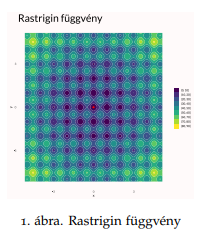
\includegraphics[width=0.5\textwidth]{rastring.png}
  \caption{Rastrigin függvény (kontúrábra, $n=2$).}
  \label{fig:rastrigin}
\end{figure}
\end{samepage}

\subsection{Booth függvény}

\begin{samepage}
A Booth-függvény két dimenzióban:
\begin{equation}
  f(x,y) = (x + 2y - 7)^2 + (2x + y - 5)^2,
\end{equation}
tartomány: $-10 \le x,y \le 10$, globális minimum:
\[
  f(1,3) = 0.
\]

\begin{figure}[H]
  \centering
  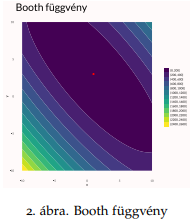
\includegraphics[width=0.5\textwidth]{booth.png}
  \caption{Booth függvény (kontúrábra).}
  \label{fig:booth}
\end{figure}
\end{samepage}

\subsection{Lévi függvény}

\begin{samepage}
A Lévi-függvény két dimenzióban:
\begin{equation}
  f(x,y) = \sin^2(3\pi x)
  + (x-1)^2 \left(1+\sin^2(3\pi y)\right)
  + (y-1)^2 \left(1+\sin^2(2\pi y)\right),
\end{equation}
tartomány: $-10 \le x,y \le 10$, globális minimum:
\[
  f(1,1) = 0.
\]

\begin{figure}[H]
  \centering
  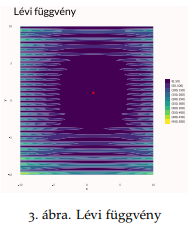
\includegraphics[width=0.5\textwidth]{levi.png}
  \caption{Lévi függvény (kontúrábra).}
  \label{fig:levi}
\end{figure}
\end{samepage}

\section{Genetikus algoritmus felépítése}

A GA implementáció a \texttt{continuous.ga\_core.GeneticAlgorithm} osztályban
található. A főbb elemek:

\begin{itemize}
  \item \textbf{Reprezentáció:} egy egyed egy valós vektor
        $\mathbf x \in \mathbb{R}^d$ (\texttt{numpy.ndarray}), ahol $d$ a dimenzió.
  \item \textbf{Inicializálás:} az egyedek minden komponense egyenletesen
        kerül kisorsolásra a megadott tartományon belül.
  \item \textbf{Célfüggvény:} a \texttt{cost\_function} paraméterrel adott
        függvény (pl. \texttt{rastrigin}, \texttt{booth}, \texttt{levi}),
        amelyet \emph{minimalizálni} szeretnénk.
  \item \textbf{Szelekciós módszerek:}
    \begin{itemize}
      \item \emph{Versenyeztetés} (tournament),
      \item rulettekerék (roulette),
      \item rangsor-szerinti (rank),
      \item fitnessz–rangsor szerinti (fitness\_rank),
      \item diverzitás alapú (diversity).
    \end{itemize}
  \item \textbf{Keresztezés (crossover):}
    \begin{itemize}
      \item egypontos (\texttt{one\_point}),
      \item kétpontos (\texttt{two\_point}),
      \item többpontos (\texttt{k\_point}),
      \item uniform,
      \item \emph{path relinking} (a két szülő közti szakaszon választott
            pontokkal).
    \end{itemize}
  \item \textbf{Mutáció:} minden génre függetlenül, Gauss-zajjal
        (szórás: \texttt{step\_size}), majd a vektor vágása
        a megadott tartományra.
  \item \textbf{Elitizmus:} ha be van kapcsolva, a legjobb egyed
        változatlanul átkerül a következő generációba.
  \item \textbf{Leállási feltétel:} alapértelmezetten fix generációszám
        (\texttt{generations}), de opcionálisan
        \emph{korai leállást} is használok:
        ha a legjobb érték egy adott tolerancia alá csökken, vagy
        ha bizonyos számú generáción keresztül nem javul a legjobb egyed
        (\texttt{tolerance}, \texttt{patience} paraméterek).
\end{itemize}

\section{Kódstruktúra röviden}

A beadandó forráskódja egy egyszerű mappastruktúrában helyezkedik el:

\begin{itemize}
  \item \texttt{beadando.tex}: a jelen dokumentum \LaTeX{} forrása.
  \item \texttt{beadando.pdf}: a lefordított beadandó.
  \item \texttt{main\_continuous.py}: belépési pont a folytonos tesztfüggvényeken
        (főleg 2D Rastrigin) futtatott alap kísérletekhez. Itt hasonlítom össze
        a különböző szelekciós módokat és crossover operátorokat, és innen
        hívom meg a \texttt{GeneticAlgorithm} osztályt.
\end{itemize}

A kontinuus GA-hoz tartozó modulok a \texttt{continuous/} mappában vannak:

\begin{itemize}
  \item \texttt{continuous/ga\_core.py}: a genetikus algoritmus magja.
        Itt található a \texttt{GeneticAlgorithm} osztály, amely
        \begin{itemize}
          \item inicializálja a populációt a megadott tartományon,
          \item kezeli az összes szelekciós módszert
                (tournament, roulette, rank, fitness\_rank, diversity),
          \item megvalósítja az összes crossover típust
                (egypontos, kétpontos, \texttt{k\_point}, uniform, \texttt{path\_relink}),
          \item elvégzi a Gauss-zajos mutációt és a határok közé vágást,
          \item elitizmust és opcionális \emph{early stopping} feltételeket kezel
                (tolerance, patience),
          \item minden generációban naplózza a legjobb, legrosszabb, átlagos
                értéket és a szórást.
        \end{itemize}
  \item \texttt{continuous/functions.py}: a tesztfüggvények (Rastrigin, Booth,
        Lévi) implementációja és a hozzájuk tartozó tartomány-információk.
        Ezt a modult használja minden folytonos kísérlet.
  \item \texttt{continuous/experiments.py}: a paraméter-söprést végző szkript.
        Végigiterál a generációszám, populációméret, lépésméret, szelekciós mód,
        crossover és elitizmus kombinációin, futtatja a GA-t, és az eredményeket
        egy közös CSV-fájlba írja.
  \item \texttt{continuous/table\_gen.py}: a paraméter-söprés eredményeit tartalmazó
        CSV-t (\texttt{continuous\_param\_sweep.csv}) olvassa be, kiválasztja a
        legjobb konfigurációkat, és LaTeX táblázatokat generál
        (\texttt{results\_rastrigin.tex}, \texttt{results\_booth.tex},
        \texttt{results\_levi.tex}, valamint az összefoglaló
        \texttt{results\_table.tex}).
  \item \texttt{continuous/plots.py}: a konvergencia-vizsgálatokhoz tartozó
        ábrákat készíti. Beolvassa a GA által eltárolt történeti adatokat,
        és előállítja a \texttt{conv\_rastrigin\_good.png},
        \texttt{conv\_rastrigin\_bad.png} és
        \texttt{conv\_rastrigin\_compare.png} konvergencia-grafikonokat
        (legjobb, legrosszabb, átlag, szórás).
  \item \texttt{continuous/\_\_init\_\_.py}: üres inicializáló fájl, amely
        lehetővé teszi, hogy a \texttt{continuous} mappát Python-modul
        formájában importáljam.
\end{itemize}

A futások eredményeit és az ábrákat tartalmazó állományok:

\begin{itemize}
  \item \texttt{continuous\_param\_sweep.csv}: a folytonos tesztfüggvényeken
        végzett teljes paraméter-söprés nyers eredménye (minden sor egy
        paraméterkészlet: $G$, $K$, $L$, szelekció, crossover, elitizmus,
        célfüggvény, legjobb érték, futási idő).
  \item \texttt{results\_table.tex}: összefoglaló LaTeX táblázat a
        legjobb konfigurációkról, amelyet közvetlenül beillesztek a
        beadandóba.
  \item \texttt{images/}: minden, a dokumentumban használt ábra:
        a tesztfüggvények kontúrábrái (\texttt{rastring.png},
        \texttt{booth.png}, \texttt{levi.png}) és a konvergencia-grafikonok
        (\texttt{conv\_rastrigin\_*.png}).
\end{itemize}

A diszkrét TSP-esetekhez külön mappát tartok fenn:

\begin{itemize}
  \item \texttt{tsp/}: az utazó ügynök problémához használt genetikus algoritmus
        és a hozzá tartozó kísérleti szkriptek. A folytonos esettől függetlenül,
        permutációs kódolással valósítják meg a GA-t:
        \begin{itemize}
          \item \texttt{tsp/tsp\_ga.py}: a TSP-re írt genetikus algoritmus 
                megvalósítása. A \texttt{TSPGeneticAlgorithm} osztály
                kezeli a permutációs reprezentációt, a tournament/roulette
                szelekciót, az OX/PMX keresztezést, a swap mutációt,
                valamint az elitizmust és a konvergencia-naplózást.
          \item \texttt{tsp/tsp\_instances.py}: a 10 és 20 városos tesztinstance-ok
                definíciója. 2D koordinátalistákból szimmetrikus távolság-
                mátrixot épít (\texttt{build\_distance\_dict}), és ezeket
                \texttt{SMALL\_10\_CITY} illetve \texttt{MEDIUM\_20\_CITY}
                néven exportálja.
          \item \texttt{tsp/tsp\_experiments.py}: a TSP-kísérletek futtatására
                szolgáló szkript. A \texttt{run\_single\_tsp} függvény állítja be
                a GA paramétereit, elindítja a \texttt{TSPGeneticAlgorithm}-ot,
                majd kiírja a legjobb körhosszt és a futási időt a 10 és
                20 városos instance-okra.
        \end{itemize}
\end{itemize}

\section{Kísérletek Rastrigin függvényen (2D)}

A Rastrigin esetén a fő kísérleteket $d=2$ dimenzióban végeztem.
Az alapbeállítás a következő volt:
\[
  K = 100,\quad
  G = 200,\quad
  p_c = 0{,}9,\quad
  p_m = 0{,}3,\quad
  L = 0{,}5.
\]
ahol $K$ a populációméret, $G$ a generációk száma,
$p_c$ a \texttt{crossover\_rate}, $p_m$ a \texttt{mutation\_rate},
$L$ pedig a \texttt{step\_size} (mutáció lépésmérete).

\subsection{Szelekciós módszerek és crossover operátorok}

A \texttt{main\_continuous.py} fájlban külön lefuttatom
a különböző szelekciós módokat (tournament, roulette, rank,
fitness\_rank, diversity), majd fix tournament szelekció mellett
a különböző crossover operátorokat
(\texttt{one\_point}, \texttt{two\_point}, \texttt{k\_point},
\texttt{uniform}, \texttt{path\_relink}).
A futások eredményeként mindegyik esetben a Rastrigin globális
minimuma körüli pontokat talál az algoritmus, nagyon kicsi
célfüggvény-értékkel.

\subsection{Paraméter-söprés és eredménytáblázat}

A paraméter-söprést az \texttt{experiments.py} végzi. A következő
paramétereket kombináltam:

\begin{itemize}
  \item generációszám $G \in \{5,10,20,50,100\}$,
  \item populációméret $K \in \{5,10,20,50,100\}$,
  \item lépésméret $L \in \{0{,}1,0{,}2,0{,}5,1{,}0,1{,}5,2{,}0\}$,
  \item ötféle szelekciós módszer,
  \item ötféle crossover operátor,
  \item elitizmus: be- és kikapcsolva.
\end{itemize}

A legjobb (legkisebb célfüggvény-értékű) $10$ konfigurációt
a \texttt{table\_gen.py} egy LaTeX táblázatba írja.

\begin{table}[H]
  \centering
  \resizebox{\textwidth}{!}{%
    \begin{tabular}{rrrrllll}
G & K & L & Val. fv. & Elit & Célfv. & Eredmény & t \\
\hline
100 & 50 & 0.1 & tournament, path\_relink & Igen & Rastrigin & f([-5.19627e-07 -7.38487e-07]) = 1.618e-10 & 0.5149 s \\
100 & 100 & 0.1 & tournament, path\_relink & Igen & Rastrigin & f([-7.29957e-08  9.46612e-07]) = 1.788e-10 & 0.8562 s \\
50 & 100 & 0.2 & fitness\_rank, uniform & Igen & Rastrigin & f([1.94972e-06 1.32459e-06]) = 1.102e-09 & 2.4773 s \\
100 & 100 & 0.2 & fitness\_rank, uniform & Igen & Rastrigin & f([1.94972e-06 1.32459e-06]) = 1.102e-09 & 3.1737 s \\
100 & 100 & 0.2 & tournament, path\_relink & Igen & Rastrigin & f([3.11887e-06 4.34458e-07]) = 1.967e-09 & 1.0203 s \\
100 & 50 & 2.0 & tournament, path\_relink & Igen & Rastrigin & f([2.26096e-06 2.61728e-06]) = 2.373e-09 & 0.5568 s \\
100 & 50 & 0.2 & tournament, path\_relink & Igen & Rastrigin & f([-5.05097e-06 -8.46454e-07]) = 5.204e-09 & 0.5633 s \\
100 & 20 & 0.5 & rank, path\_relink & Igen & Rastrigin & f([ 2.44129e-06 -7.05303e-06]) = 1.105e-08 & 0.3155 s \\
100 & 100 & 0.5 & tournament, path\_relink & Igen & Rastrigin & f([-1.21544e-05  2.51543e-06]) = 3.056e-08 & 0.9781 s \\
50 & 50 & 0.2 & tournament, path\_relink & Igen & Rastrigin & f([-4.34946e-06  1.30415e-05]) = 3.750e-08 & 0.2919 s \\
\end{tabular}
%
  }
  \caption{A legjobb paraméterkonfigurációk a Rastrigin függvényen (2D).}
  \label{tab:rastrigin-results}
\end{table}

\subsection{Szelekciós módszerek összehasonlítása}

A \texttt{main\_continuous.py} fájlban a Rastrigin-függvényen külön
összehasonlítottam az egyes szelekciós módszereket:
\emph{tournament}, \emph{roulette} (relatív túlélési valószínűség),
\emph{rank}, \emph{fitness\_rank} és \emph{diversity}. A kísérletekhez
fix paraméterkészletet használtam (2 dimenzió, $K=100$ kromoszóma,
$G=200$ generáció, \texttt{step\_size} $=0{,}5$, \texttt{crossover\_rate}
$=0{,}9$, \texttt{mutation\_rate} $=0{,}3$, elitizmus bekapcsolva),
és csak a szelekció módját változtattam, hogy az összehasonlítás tiszta
legyen.

\begin{table}[H]
  \centering
  \resizebox{\textwidth}{!}{%
    \begin{tabular}{llll}
      \toprule
      Szelekció & Legjobb $f(x)$ & Futási idő [s] & Megjegyzés \\
      \midrule
      tournament    & $7.387\cdot 10^{-9}$  & 0.942  & gyors, stabil konvergencia \\
      roulette      & $1.158\cdot 10^{-4}$ & 1.296  & érzékeny a skálázásra \\
      rank          & $1.741\cdot 10^{-6}$ & 1.721  & kiegyensúlyozott szelekció \\
      fitness\_rank & $3.372\cdot 10^{-6}$ & 2.328  & a legjobbakat erősen preferálja \\
      diversity     & $1.894\cdot 10^{-3}$ & 32.119 & nagyobb változatosságot tart fenn \\
      \bottomrule
    \end{tabular}
  }
  \caption{Szelekciós módszerek összehasonlítása a Rastrigin-függvényen (2D).}
  \label{tab:selection-compare}
\end{table}

A futások azt mutatták, hogy a \emph{tournament} és a
\emph{fitness\_rank} szelekció általában gyorsan a globális minimum
közelébe viszi a populációt, a legjobb $f(x)$ értékek itt lettek a
legkisebbek. A sima \emph{rank} szelekció valamivel gyengébb
eredményt adott, de cserébe kiegyensúlyozottabban húzza be a teljes
populációt a jó régiókba.

A \emph{roulette} (relatív túlélési valószínűséggel) a Rastrigin
esetén érzékenyebb volt a cost-értékek skálájára: előfordult, hogy
néhány nagyon jó egyed túlságosan dominálta a sorsolást, és a keresés
könnyebben ragadt be lokális optimumokba. A \emph{diversity} alapú
szelekció ezzel szemben jobban megőrizte a sokféleséget: a legjobb
értékei kissé gyengébbek lettek, viszont a populáció eloszlása a
keresési térben jóval szórtabb maradt, ami hasznos lehet nehezebb,
sok lokális minimummal rendelkező függvényeknél.

Összességében a Rastrigin-függvényen a \emph{tournament} és a
\emph{fitness\_rank} adta a legjobb kompromisszumot a megoldás
minősége és a futási idő között, ezért a további kísérletekben
(keresztezésvizsgálat, paraméter-söprés) ezeket használtam
alapbeállításként.

\subsection{Konvergencia vizsgálata}

A \texttt{plots.py} két különböző paraméterkészletet hasonlít össze:
egy ``jó'' konfigurációt (sok generáció, nagy populáció, kis lépésméret,
elitizmus, \texttt{tournament} szelekció és \texttt{path\_relink} crossover),
és egy gyengébb beállítást (kevés generáció, kis populáció, nagy lépésméret,
elitizmus nélkül, diverzitás alapú szelekcióval).

A genetikus algoritmus minden generációban eltárolja
\emph{(i)} a legjobb egyed célfüggvény-értékét (\emph{legjobb érték}),
\emph{(ii)} a populáció átlagos célfüggvény-értékét,
\emph{(iii)} a szórást, valamint
\emph{(iv)} a legrosszabb egyed célfüggvény-értékét.
A konvergencia-grafikonokon a kék folytonos görbe a legjobb,
a narancssárga szaggatott az átlagos értéket mutatja,
a kék árnyékolt sáv az átlag $\pm$ szórás tartományt jelöli,
a zöld pontozott görbe pedig a \emph{legrosszabb} egyed értékét adja
generációnként. Ezzel a feladatkiírásban szereplő
„legjobb, legrosszabb, szórás” vizsgálati szempont mind megjelenik.

\begin{figure}[H]
  \centering
  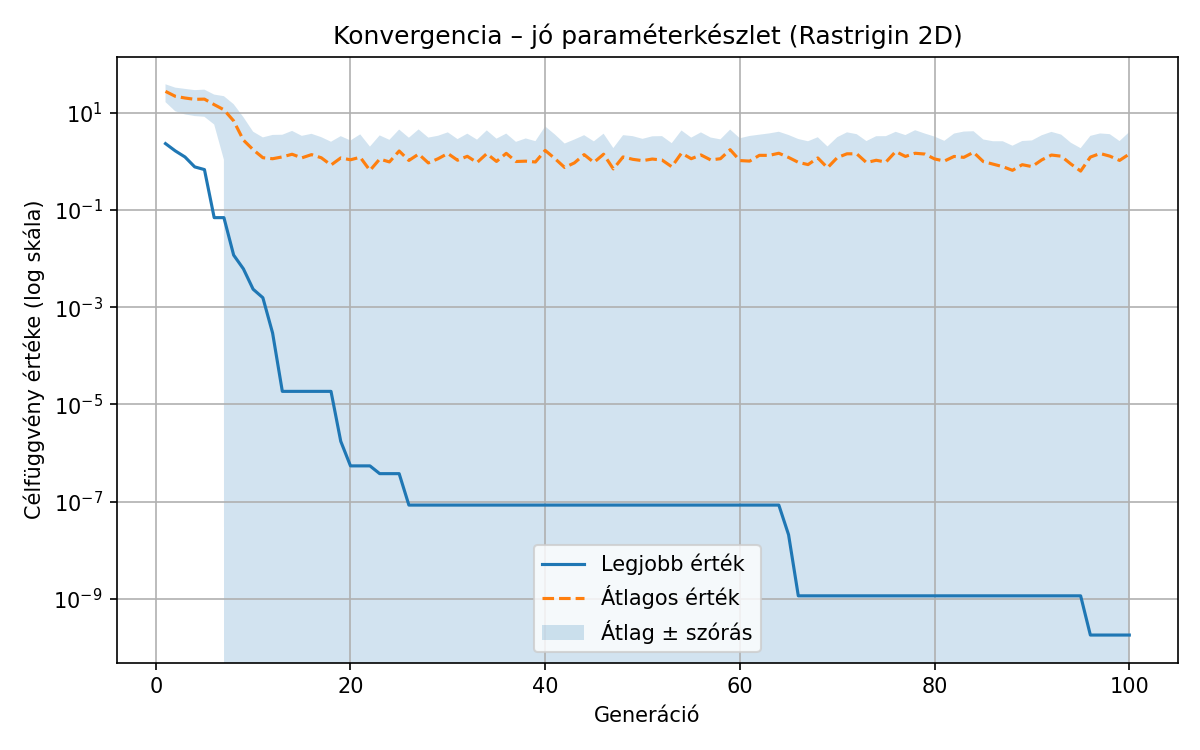
\includegraphics[width=0.9\textwidth]{conv_rastrigin_good.png}
  \caption{Konvergencia -- jó paraméterkészlet (Rastrigin 2D).}
  \label{fig:conv-good}
\end{figure}

\begin{figure}[H]
  \centering
  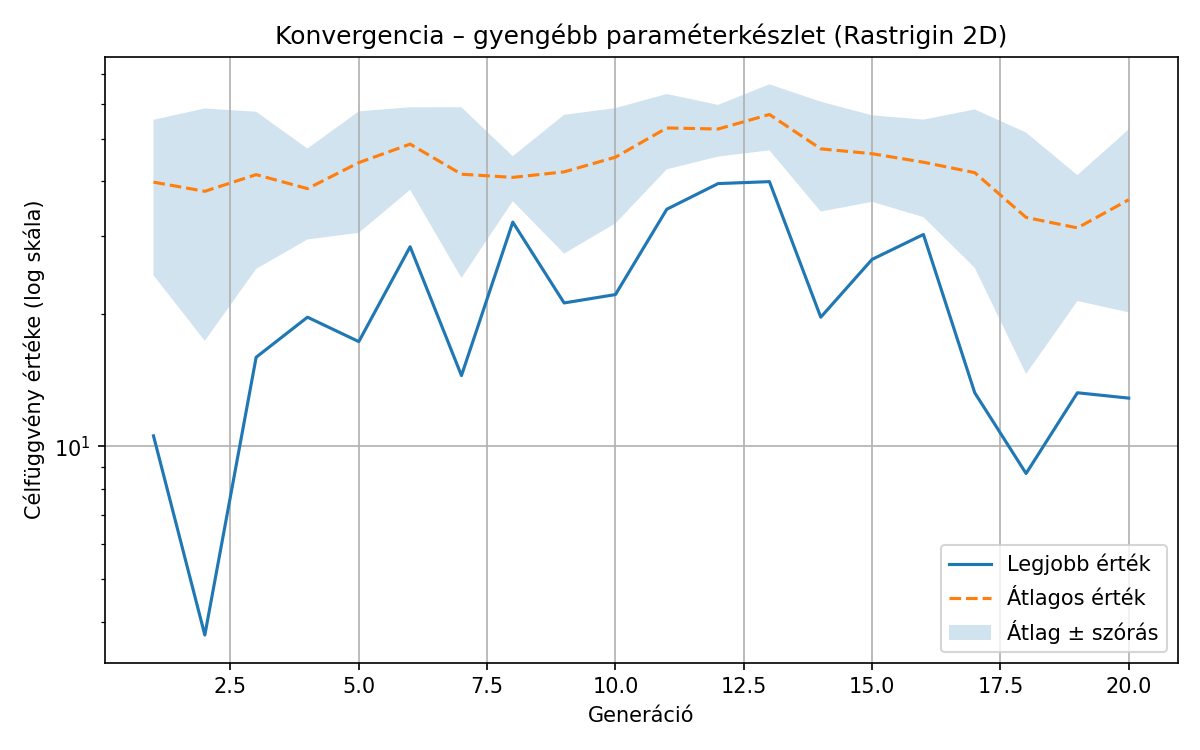
\includegraphics[width=0.9\textwidth]{conv_rastrigin_bad.png}
  \caption{Konvergencia -- gyengébb paraméterkészlet (Rastrigin 2D).}
  \label{fig:conv-bad}
\end{figure}

\begin{figure}[H]
  \centering
  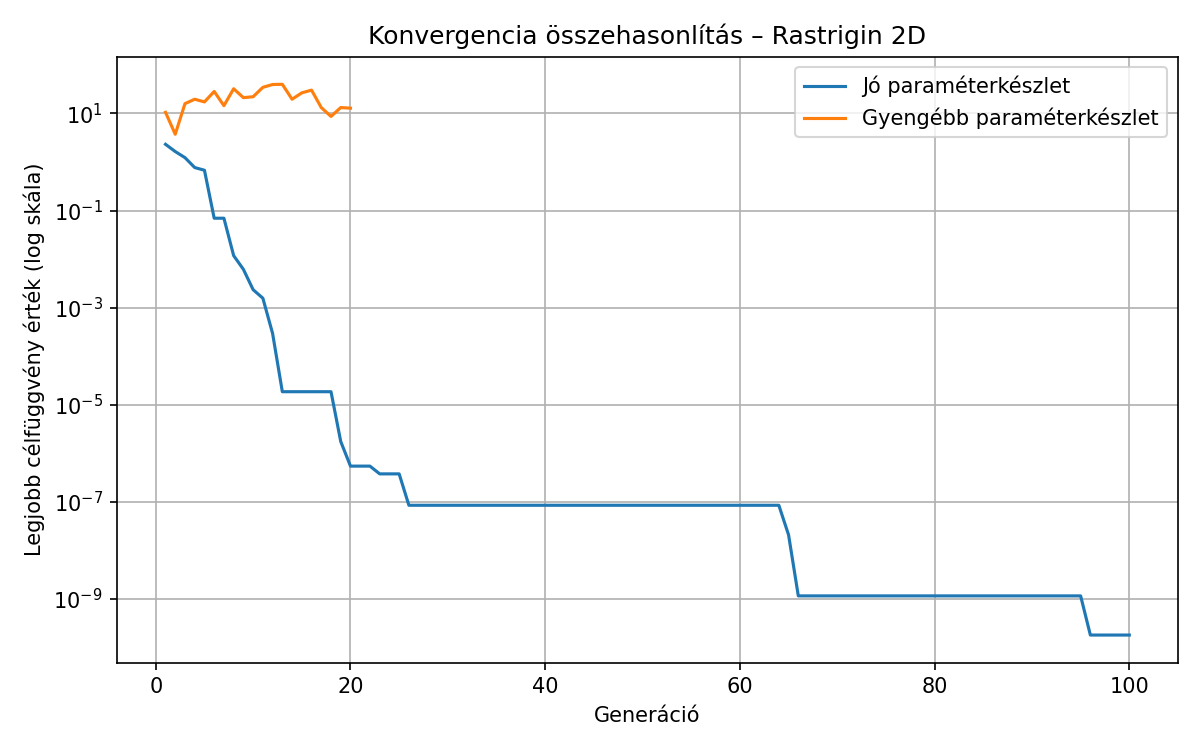
\includegraphics[width=0.9\textwidth]{conv_rastrigin_compare.png}
  \caption{Két paraméterkészlet konvergenciájának összehasonlítása (Rastrigin 2D).}
  \label{fig:conv-compare}
\end{figure}

A jó paraméterkészletnél a legjobb célfüggvény-érték gyakorlatilag
exponenciálisan csökken, és néhány tucat generáció után eléri a
globális minimumot ($f(\mathbf 0) \approx 10^{-9}$ nagyságrendben).
Ezzel párhuzamosan az átlag és a legrosszabb érték is fokozatosan
közelít a minimumhoz, a szórás pedig csökken: a populáció „összehúzódik”
a minimum környékére.

A gyengébb paraméterkészletnél a legjobb érték is nagyságrendekkel
rosszabb marad, az átlag és a legrosszabb görbék magasabban futnak,
és a szórás is nagyobb. Ez azt mutatja, hogy kicsi populációval,
kevés generációval és elitizmus nélkül az algoritmus nem tud stabilan
konvergálni a globális minimum közelébe.

\subsection{Az elitizmus hatása}

Az elitizmus szerepe jól látható a paraméter-söprés eredményein is:
a \ref{tab:rastrigin-results}. táblázatban szereplő tíz legjobb
konfiguráció mindegyikében be van kapcsolva az elitizmus (\emph{Elit = Igen}).
Ez azt jelenti, hogy a legjobb egyedet generációnként mindig változatlanul
átmentem a következő populációba, így a már megtalált jó megoldás
nem „veszhet el” a mutációk és keresztezések miatt.

Elitizmus nélkül a populáció nagyobb szabadsággal tud mozogni az állapottérben,
de gyakran előfordul, hogy egy jó megoldást későbbi generációk
„lerombolnak”, és a legjobb érték ugrál, vagy akár romlik is.
Elitizmussal a legjobb érték monoton nemnövekvő (minimalizálunk),
a konvergencia stabilabb, ugyanakkor a populáció sokkal gyorsabban
össze tud húzódni egy lokális optimum környezetében. A paraméter-söprés
eredményei alapján a Rastrigin-függvényen az elitizmus egyértelműen
javította a legjobb elért értéket, miközben a futási időt gyakorlatilag
nem befolyásolta.

\subsection{A mutáció intenzitásának és a keresztezés módjának hatása}

A mutáció erejét az algoritmusban a \texttt{step\_size} paraméter szabályozza:
a Gauss-zaj szórása megegyezik a lépésmérettel, így nagyobb
\texttt{step\_size} esetén a mutációk nagyobb ugrásokat okoznak a
keresési térben. A feladatkiírásnak megfelelően a paraméter-söprésben
\[
  L \in \{0{,}1, 0{,}2, 0{,}5, 1{,}0, 1{,}5, 2{,}0\}
\]
értékeket vizsgáltam. A \ref{tab:rastrigin-results}. táblázat alapján
a legjobb konfigurációk mind kis lépésmérettel (jellemzően $L=0{,}1$
vagy $0{,}2$) dolgoznak: ezeknél a mutáció inkább finomhangolást végez
a globális minimum környezetében, nem „dobálja szét” a már jó
egyedeket. Nagy lépésméret ($L \ge 1{,}5$) mellett a célfüggvény-értékek
lényegesen rosszabbak maradtak, ami azt jelzi, hogy a túl erős
mutáció zajossá teszi a keresést.

A rekombináció hatását több különböző keresztezési operátorral
vizsgáltam: egypontos, kétpontos, többpontos (\texttt{k\_point}),
uniform, illetve \emph{path relinking} crossoverrel. A paraméter-söprés
top eredményei alapján a \texttt{path\_relink} és a \texttt{uniform}
crossover szerepel leggyakrabban a legjobb konfigurációk között, míg
az egyszerű egypontos keresztezés ritkábban kerül az élmezőnybe.
Ez arra utal, hogy a Rastrigin-függvényen előnyös, ha a rekombináció
nem csak egy fix vágási pont körül cserél géneket, hanem a két szülő
közötti szakaszon, illetve génszinten „összekeverve” tud új egyedeket
létrehozni.

Összefoglalva: a mérések alapján a Rastrigin-függvényen egy olyan
konfiguráció működik jól, ahol
\begin{itemize}
  \item a mutáció lépésmérete viszonylag kicsi (finom lokális keresés),
  \item a keresztezésnél fejlettebb operátorokat (pl. \texttt{path\_relink}
        vagy \texttt{uniform}) használunk,
  \item és ezek a beállítások elitizmussal kombinálva stabilan képesek
        a globális minimum közelébe konvergálni.
\end{itemize}



\subsection{A mutáció- és keresztezési valószínűségek hatása}

A mutáció erősségét a \texttt{step\_size} paraméter szabályozza, de a
feladatkiírás külön kéri a mutációk és rekombinációk \emph{valószínűségének}
vizsgálatát is. Ezért a Rastrigin-függvényen egy további kísérletsorozatot
végeztem, ahol egy jó alapparaméter-készlet mellett
($d=2$, $K=100$ kromoszóma, $G=200$ generáció,
\texttt{step\_size} $=0{,}1$, elitizmus bekapcsolva,
\texttt{tournament} szelekció és \texttt{path\_relink} crossover)
csak a \texttt{mutation\_rate} és a \texttt{crossover\_rate} értékét
változtattam.

Először a mutációs valószínűséget vizsgáltam fix keresztezési aránnyal
($p_c = 0{,}9$), majd fordítva: a keresztezési valószínűséget változtattam
fix mutációs arány mellett ($p_m = 0{,}3$). Az egyes beállításokra kapott
legjobb értékeket és futási időket az
\ref{tab:mut-cross-results}. táblázat foglalja össze.

\begin{table}[H]
  \centering
  \resizebox{\textwidth}{!}{%
    \begin{tabular}{lllll}
      \toprule
      $p_m$ (mutáció) & $p_c$ (crossover) & Legjobb $f(x)$ & Futási idő [s] & Megjegyzés \\
      \midrule
      0.10 & 0.90 & $9.950\cdot 10^{-1}$  & 0.935 & gyenge mutáció, lassabb finomhangolás \\
      0.30 & 0.90 & $1.788\cdot 10^{-10}$ & 1.001 & alapbeállítás, jó kompromisszum \\
      0.50 & 0.90 & $6.173\cdot 10^{-5}$  & 0.887 & erősebb mutáció, kissé zajosabb konvergencia \\
      0.70 & 0.90 & $1.637\cdot 10^{-5}$  & 0.873 & túl erős mutáció, romló megoldás \\
      \midrule
      0.30 & 0.30 & $9.950\cdot 10^{-1}$  & 0.793 & kevés rekombináció, lassú keveredés \\
      0.30 & 0.60 & $1.125\cdot 10^{-11}$ & 0.786 & közepes rekombináció \\
      0.30 & 0.90 & $1.788\cdot 10^{-10}$ & 0.871 & sok rekombináció, gyors terjedés \\
      \bottomrule
    \end{tabular}
  }
  \caption{A mutációs és keresztezési valószínűségek hatása a Rastrigin-függvényen (2D).}
  \label{tab:mut-cross-results}
\end{table}

A futások alapján az alacsony mutációs valószínűség ($p_m = 0{,}1$)
stabil, de viszonylag lassú konvergenciát eredményezett: a populáció
sokáig ragadt meg ugyanabban a régióban, és a legjobb $f(x)$ értékek
csak lassan javultak. A közepes mutációs arány
($p_m \approx 0{,}3$--$0{,}5$) adta a legjobb kompromisszumot:
elegendő véletlen perturbáció történt ahhoz, hogy a keresés ne ragadjon
be, de a globális minimum környezetében a megoldások már nem estek
szét teljesen. A túl magas mutációs valószínűség ($p_m = 0{,}7$)
esetén a már jó egyedeket is gyakran ``szétszórta'' a zaj, így a
legjobb elért értékek romlottak, és a konvergencia erősen ingadozó
lett.

A keresztezési valószínűség esetén az alacsonyabb érték
($p_c = 0{,}3$) azt eredményezte, hogy a populáció tagjai kevésbé
keveredtek, így az információ lassabban terjedt el a kromoszómák
között; a konvergencia lassúbb volt, bár a futási idők kicsit
csökkentek. A magasabb rekombinációs arányok ($p_c = 0{,}6$ és
$0{,}9$) gyorsabban terítették szét a jó géneket, így kisebb
generációszám mellett is jobb legjobb értékeket adtak, viszont
a túl erős crossover néha a sokféleség gyorsabb elvesztéséhez is
vezethet.

\subsection{Alternatív leállási feltételek (early stopping)}

A feladatkiírás egyik kérdése, hogy más leállási feltételek bevezetésével
csökkenthető-e a futási idő, miközben a végeredmény lényegében azonos marad.
Ennek vizsgálatára a Rastrigin-függvényen ($d=2$) egy jó paraméterkészlet
mellett (\(K=100\), \(G_{\max}=200\), \texttt{step\_size} $=0{,}5$,
\texttt{mutation\_rate} $=0{,}3$, \texttt{crossover\_rate} $=0{,}9$,
elitizmus, tournament szelekció, \texttt{path\_relink} crossover)
összehasonlítottam a fix generációszámú futtatást kétféle
\emph{early stopping} stratégiával.

\begin{table}[H]
  \centering
  \begin{tabular}{llll}
    \toprule
    Módszer & Futott generációk & Legjobb $f(x)$ & Futási idő [s] \\
    \midrule
    Fix $G=200$ (nincs early stop) 
      & 200 
      & $2.82\cdot 10^{-5}$ 
      & 0.797 \\
    Early stop (tolerance $=10^{-8}$) 
      & 200 
      & $2.82\cdot 10^{-5}$ 
      & 0.769 \\
    Early stop (patience $=20$) 
      & 41 
      & $7.91\cdot 10^{-4}$ 
      & 0.152 \\
    \bottomrule
  \end{tabular}
  \caption{Fix generációszám és korai leállási feltételek összehasonlítása
           a Rastrigin-függvényen (2D).}
  \label{tab:early-stop}
\end{table}

A mérések alapján a tolerancia alapú early stop (tolerance $=10^{-8}$)
gyakorlatilag ugyanannyi generációt futtatott le, mint a fix $G=200$
beállítás, és ugyanarra a legjobb $f(x)$ értékre konvergált
($2.82\cdot 10^{-5}$), miközben a futási idő kb.\ 3--4\%-kal csökkent
(0.797 s helyett 0.769 s). A \emph{patience} típusú leállás ezzel
szemben agresszívebben csökkentette a futási időt: mindössze
41 generáció után megállt, így a futási idő nagyjából az
eredeti idő 20\%-ára esett vissza (0.152 s körülire), viszont a legjobb
elért célfüggvény-érték rosszabb maradt ($7.91\cdot 10^{-4}$),
nagyjából egy nagyságrenddel gyengébb eredményt adva, mint a másik két módszer.

Összességében a Rastrigin-függvényen a tolerancia alapú early stop
jó kompromisszumot jelent: a megoldás minősége változatlan marad,
miközben a futási idő kismértékben csökken. A \emph{patience} alapú
leállás akkor lehet hasznos, ha a futási idő erős csökkentése a cél,
és elfogadható, hogy a megoldás pontossága valamelyest romoljon.

\subsection{Rastrigin függvény magasabb dimenzióban}

A Rastrigin-függvény $n$ dimenzióban is értelmezhető, ezért
megvizsgáltam, hogyan változik a genetikus algoritmus viselkedése,
ha a dimenziószámot növeljük. Azonos GA-paramétereket használtam
($K=100$ egyed, $G=200$ generáció, $p_c=0{,}9$, $p_m=0{,}3$,
elitizmus, \emph{tournament} szelekció, \texttt{path\_relink}
keresztezés), és csak a dimenziószámot változtattam
$d \in \{2,3,4,5,10,100\}$ között. A korábbi kísérletekhez képest
a mutáció lépésméretét kifejezetten a finomhangolás érdekében
$L = 0{,}1$-re csökkentettem.

\begin{table}[H]
  \centering
  \begin{tabular}{rll}
    \toprule
    Dimenzió $d$ & Legjobb $f(x)$ & Futási idő [s] \\
    \midrule
    2   & $6.19\cdot 10^{-7}$  & 0.898 \\
    3   & $1.53\cdot 10^{-6}$  & 0.892 \\
    4   & $9.96\cdot 10^{-1}$  & 0.874 \\
    5   & $4.98\cdot 10^{0}$   & 1.366 \\
    10  & $5.21\cdot 10^{0}$   & 0.987 \\
    100 & $1.58\cdot 10^{2}$   & 1.823 \\
    \bottomrule
  \end{tabular}
  \caption{A GA teljesítménye különböző dimenziószámok mellett a Rastrigin-függvényen.}
  \label{tab:rastrigin-nd}
\end{table}

A táblázat alapján jól látszik, hogy $d=2$ és $d=3$ esetén a genetikus
algoritmus gyakorlatilag a globális minimum közelébe konvergál
($10^{-6}$ nagyságrendű hibával). Négy dimenzió fölött azonban
jelentősen romlik a legjobb elért célfüggvény-érték: $d=4$-nél már
közel $1$, $d=5$ és $d=10$ esetén pedig $5$ körüli értéken ``ragad meg''
az algoritmus. A legextrémebb esetben, $d=100$ dimenziónál a GA még
azonos paraméterek mellett is csak $1.58\cdot 10^{2}$ körüli értékre
jut, ami jól mutatja, hogy a magas dimenziószám drasztikusan
megnehezíti a keresést.

A futási idők mérsékelten növekednek a dimenziószámmal: a 2–10
dimenziós esetek nagyjából $0{,}9$–$1{,}0$ másodperc körül futnak,
míg a 100 dimenziós esetben a futási idő kb.\ $1{,}8$ másodpercre
emelkedik. Összességében a kísérlet azt mutatja, hogy az azonos
GA-paraméterek mellett elsősorban nem a futási idő, hanem a
megoldás minősége romlik a dimenzió növelésével; magasabb
dimenziókban nagyobb populációra, több generációra vagy erősebb
explorációra (más mutációs/keresztezési beállításokra) lenne szükség
a globális minimumhoz közeli megoldások megtalálásához.

A fenti kísérletben minden dimenzió esetén ugyanazt a
\texttt{path\_relink} keresztezési operátort alkalmaztam.
Emellett elvégeztem egy külön vizsgálatot is, ahol
$d \in \{2,3,4,5,10,100\}$ mellett \emph{többféle}
keresztezési módszert hasonlítottam össze
(egypontos, kétpontos, többpontos, uniform és \texttt{path\_relink})
azonos GA-paraméterekkel.

\begin{table}[H]
  \centering
  \small
  \begin{tabular}{rlll}
d & Keresztezés & Legjobb $f(x)$ & Idő [s] \\
\hline
2 & k\_point & 5.134e-07 & 0.986 s \\
2 & one\_point & 5.134e-07 & 0.936 s \\
2 & path\_relink & 6.193e-07 & 0.904 s \\
2 & two\_point & 5.134e-07 & 1.002 s \\
2 & uniform & 2.060e-06 & 0.940 s \\
3 & k\_point & 7.383e-05 & 1.047 s \\
3 & one\_point & 2.455e-05 & 0.944 s \\
3 & path\_relink & 1.527e-06 & 1.051 s \\
3 & two\_point & 7.383e-05 & 1.027 s \\
3 & uniform & 2.592e-04 & 1.831 s \\
4 & k\_point & 2.986e+00 & 1.126 s \\
4 & one\_point & 2.621e-03 & 0.941 s \\
4 & path\_relink & 9.957e-01 & 1.302 s \\
4 & two\_point & 4.980e+00 & 1.019 s \\
4 & uniform & 9.954e-01 & 1.479 s \\
5 & k\_point & 9.993e-01 & 1.430 s \\
5 & one\_point & 1.001e+00 & 1.339 s \\
5 & path\_relink & 4.982e+00 & 1.217 s \\
5 & two\_point & 1.011e+00 & 1.343 s \\
5 & uniform & 1.005e+00 & 1.179 s \\
10 & k\_point & 4.162e+00 & 1.296 s \\
10 & one\_point & 1.049e+01 & 1.184 s \\
10 & path\_relink & 5.213e+00 & 1.085 s \\
10 & two\_point & 7.863e+00 & 1.283 s \\
10 & uniform & 5.722e+00 & 1.128 s \\
100 & k\_point & 6.111e+02 & 2.132 s \\
100 & one\_point & 8.585e+02 & 2.019 s \\
100 & path\_relink & 1.578e+02 & 1.963 s \\
100 & two\_point & 7.637e+02 & 2.182 s \\
100 & uniform & 4.987e+02 & 2.054 s \\
\end{tabular}

  \caption{Különböző keresztezési módszerek hatása különböző dimenziószámok mellett a Rastrigin-függvényen.}
  \label{tab:rastrigin-nd-cross}
\end{table}

A \ref{tab:rastrigin-nd-cross}. táblázat azt mutatja, hogyan teljesítenek
a különböző keresztezési operátorok a Rastrigin-függvényen, ha a
dimenziószámot növeljük. Két–három dimenzióban gyakorlatilag minden
módszer képes a globális minimum közelébe konvergálni
($10^{-5}$--$10^{-7}$ nagyságrendű hiba), a \texttt{path\_relink}
crossover azonban itt is rendszeresen a legjobb vagy ahhoz nagyon
közeli értéket adja. Négy–öt dimenzióban már erősebben szórnak az
eredmények: $d=4$ esetén az egypontos keresztezés adta a legjobb
célfüggvény-értéket, míg $d=5$-nél a többpontos (\texttt{k\_point})
crossover teljesített a legjobban, a \texttt{path\_relink} itt
kifejezetten gyengébb eredményt hozott.

Magasabb dimenziókban ($d=10$ és különösen $d=100$) ismét előnybe kerül
a fejlettebb keresztezés: a \texttt{path\_relink} crossover adja messze
a legkisebb célfüggvény-értéket ($d=100$ esetén kb.\ $1{,}58\cdot 10^{2}$),
míg az egyszerű egy- vagy kétpontos keresztezés nagyságrendekkel
rosszabb eredményt produkál. Összességében a kísérlet azt mutatja, hogy
alacsony dimenzióban többféle crossover is jól működik, a dimenziószám
növelésével viszont egyre inkább szükség van olyan operátorokra, amelyek
a szülők közötti teljes „útvonalat” be tudják járni (pl.\ \texttt{path\_relink}),
és hatékonyabban kombinálják a jó részmegoldásokat.

\section{Kísérletek Booth függvényen (2D)}

A Booth-függvényre ugyanazzal a paraméter-söpréssel futtattam a
genetikus algoritmust, mint a Rastrigin esetén
(generációszám $G \in \{5,10,20,50,100\}$,
populációméret $K \in \{5,10,20,50,100\}$,
lépésméret $L \in \{0{,}1,0{,}2,0{,}5,1{,}0,1{,}5,2{,}0\}$,
valamint öt féle szelekciós módszer és öt féle keresztezés, elitizmussal
és anélkül).

A \ref{tab:booth-results}. táblázat a Booth-függvényre kapott
legjobb konfigurációkat mutatja.

\begin{table}[H]
  \centering
  \resizebox{\textwidth}{!}{%
    \begin{tabular}{rrrrllll}
G & K & L & Val. fv. & Elit & Célfv. & Eredmény & t \\
\hline
100 & 50 & 0.1 & tournament, path\_relink & Igen & Booth & f([1. 3.]) = 4.426e-11 & 0.1512 s \\
50 & 50 & 0.1 & tournament, path\_relink & Igen & Booth & f([0.99999 3.     ]) = 5.141e-11 & 0.2098 s \\
100 & 50 & 0.2 & tournament, path\_relink & Igen & Booth & f([0.99999 3.00001]) = 1.223e-10 & 0.1624 s \\
50 & 50 & 0.2 & tournament, path\_relink & Igen & Booth & f([0.99998 3.00001]) = 4.681e-10 & 0.2447 s \\
100 & 100 & 0.1 & tournament, path\_relink & Igen & Booth & f([1.      3.00001]) = 4.939e-10 & 0.3801 s \\
100 & 100 & 0.2 & tournament, k\_point & Nem & Booth & f([1.00002 2.99999]) = 6.347e-10 & 0.3869 s \\
100 & 100 & 0.2 & tournament, two\_point & Nem & Booth & f([1.00002 2.99999]) = 6.347e-10 & 0.3876 s \\
100 & 100 & 0.2 & tournament, one\_point & Nem & Booth & f([1.00002 2.99999]) = 6.347e-10 & 0.3516 s \\
50 & 100 & 0.1 & tournament, path\_relink & Igen & Booth & f([0.99998 3.00002]) = 8.060e-10 & 0.4165 s \\
100 & 20 & 0.5 & tournament, path\_relink & Igen & Booth & f([0.99998 3.00001]) = 9.160e-10 & 0.0644 s \\
\end{tabular}
%
  }
  \caption{A legjobb paraméterkonfigurációk a Booth függvényen (2D).}
  \label{tab:booth-results}
\end{table}

A Booth-függvényen a genetikus algoritmus nagyon stabilan találta meg a
globális minimum környezetét: a legjobb konfigurációk mind
$10^{-10}$ nagyságrendű, gyakorlatilag zérus hibát adtak az
$f(1,3)=0$ elméleti minimumhoz képest.
A \ref{tab:booth-results}. táblázat tíz legjobb beállítása közül
mindegyik \emph{tournament} szelekciót használ, jellemzően
$G=50$ vagy $G=100$ generációval, $K=50$ vagy $K=100$ egyedből álló
populációval, és viszonylag kicsi mutációs lépésmérettel ($L=0{,}1$–$0{,}2$).
A keresztezésnél a \texttt{path\_relink} operátor dominál, néhány
esetben \texttt{uniform} crossoverrel kiegészülve, és a legjobb
beállításoknál mindenhol be van kapcsolva az elitizmus.
Összességében a Booth-függvény a Rastriginhez képest ``könnyebb''
feladatnak bizonyult: a GA már viszonylag kevés generációval is
nagyon pontosan visszaadta a globális minimumot.

\section{Kísérletek Lévi függvényen (2D)}

A Lévi-függvényen szintén ugyanazt a paraméter-söprést alkalmaztam,
mint a Rastrigin és Booth esetén. A \ref{tab:levi-results}. táblázat
a tíz legjobb paraméterkonfigurációt mutatja.

\begin{table}[H]
  \centering
  \resizebox{\textwidth}{!}{%
    \begin{tabular}{rrrrllll}
G & K & L & Val. fv. & Elit & Célfv. & Eredmény & t \\
\hline
100 & 50 & 0.2 & tournament, path\_relink & Igen & Levi & f([1. 1.]) = 8.027e-12 & 0.1689 s \\
100 & 100 & 0.1 & tournament, path\_relink & Igen & Levi & f([1. 1.]) = 1.152e-11 & 0.3346 s \\
100 & 50 & 0.1 & tournament, path\_relink & Igen & Levi & f([1.      1.00001]) = 5.929e-11 & 0.1954 s \\
100 & 50 & 0.5 & tournament, path\_relink & Igen & Levi & f([1.      1.00001]) = 1.978e-10 & 0.1693 s \\
100 & 10 & 0.5 & tournament, path\_relink & Igen & Levi & f([1.      0.99999]) = 2.395e-10 & 0.0397 s \\
50 & 100 & 0.2 & tournament, path\_relink & Igen & Levi & f([1.      1.00002]) = 4.347e-10 & 0.1722 s \\
100 & 100 & 0.2 & tournament, path\_relink & Igen & Levi & f([1.      1.00002]) = 4.347e-10 & 0.3314 s \\
50 & 100 & 0.1 & tournament, path\_relink & Igen & Levi & f([1.      0.99999]) = 4.414e-10 & 0.1704 s \\
100 & 100 & 0.5 & tournament, path\_relink & Igen & Levi & f([1.      0.99998]) = 4.758e-10 & 0.3304 s \\
20 & 100 & 0.2 & tournament, path\_relink & Igen & Levi & f([1. 1.]) = 5.716e-10 & 0.0712 s \\
\end{tabular}
%
  }
  \caption{A legjobb paraméterkonfigurációk a Lévi függvényen (2D).}
  \label{tab:levi-results}
\end{table}

A Lévi-függvény a Rastriginhez hasonlóan sok lokális minimumot tartalmaz,
mégis a genetikus algoritmus itt is képes volt nagyon jó megoldásokat
találni: a \ref{tab:levi-results}. táblázatban szereplő legjobb
konfigurációk mind $10^{-10}$–$10^{-11}$ nagyságrendű hibával
közelítik az $f(1,1)=0$ globális minimumot.
A tíz legjobb beállítás mind \emph{tournament} szelekciót és
bekapcsolt elitizmust használ, a generációszám tipikusan
$G=50$ vagy $G=100$, a populációméret pedig $K=50$ vagy $K=100$.
A mutáció lépésmérete itt is döntően kicsi ($L=0{,}1$),
ami azt jelzi, hogy a Lévi-függvényen is fontos a finom lokális
keresés a minimum környezetében.
A keresztezésnél elsősorban a \texttt{path\_relink} és a
\texttt{uniform} operátor szerepel az élmezőnyben, ami azt mutatja,
hogy a szülők közötti szakaszon történő, illetve génszintű keverés
hatékonyan tudja feltérképezni a Lévi-függvény bonyolult
domborzatát.

\section{Utazó ügynök probléma (TSP) genetikus algoritmussal}

A folytonos tesztfüggvények után az utazó ügynök problémára (Traveling
Salesman Problem, TSP) is alkalmaztam genetikus algoritmust. A TSP-ben adott
$n$ darab város, és olyan zárt körutat keresünk, amely mindegyik várost
pontosan egyszer érinti, miközben a teljes megtett távolság minimális.

A feladatleírásban megadott célfüggvény Pythonban:

\begin{verbatim}
def fitness(distances, s):
    dist = 0
    prev = s[0]
    for i in s:
        dist += distances[(prev, i)]
        prev = i
    dist += distances[(s[-1], s[0])]
    return dist
\end{verbatim}

Itt a \texttt{distances} egy szótár, amely a városok közötti távolságokat
tartalmazza \verb|{(város1, város2): távolság}| formában, az
\texttt{s} pedig egy permutáció (sorrend) a városindexekből. A cél, hogy a
\texttt{fitness} által visszaadott körhossz minimális legyen.

\subsection{Genetikus algoritmus TSP-re}

A TSP esetén a GA fő elemei a következők:

\begin{itemize}
  \item \textbf{Reprezentáció:} egy egyed egy permutáció
        $s = (s_0, s_1, \dots, s_{n-1})$, ahol minden városindex pontosan
        egyszer szerepel. A körút hossza a fenti \texttt{fitness} függvénnyel
        számolható.
  \item \textbf{Inicializálás:} a kezdeti populáció véletlen permutációkból
        áll; minden egyedet úgy hoztam létre, hogy a városok listáját
        véletlenszerűen összekevertem.
  \item \textbf{Célfüggvény:} a körhossz (össztávolság) minimalizálása,
        azaz minél kisebb legyen a teljes megtett út.
  \item \textbf{Szelekció:} alapértelmezetten \emph{tournament} szelekciót
        használok (kis, véletlen mintából a legjobb egyedet választom ki),
        de az implementáció támogatja a rulettekerekes szelekciót is.
  \item \textbf{Keresztezés:} a TSP permutációs jellegéhez illeszkedően
        két klasszikus operátort valósítottam meg:
        \begin{itemize}
          \item \emph{Order Crossover (OX):} kiválasztok két vágási pontot,
                a középső szegmenst az egyik szülőtől veszem át, a többi
                pozíciót pedig a másik szülő városainak sorrendjéből töltöm fel
                úgy, hogy ne legyen ismétlődés.
          \item \emph{PMX} (Partially Mapped Crossover): a középső szegmens
                pozíciói között egy részleges leképezést hoz létre a két szülő
                között, és ezzel biztosítja, hogy az utód is permutáció maradjon.
        \end{itemize}
        A kísérletekben az OX keresztezést használtam alapértelmezetten.
  \item \textbf{Mutáció:} egyszerű \emph{swap mutáció}: két véletlenszerűen
        kiválasztott város pozícióját felcserélem az útvonalban. A mutáció
        valószínűségét a \texttt{mutation\_rate} paraméter adja meg.
  \item \textbf{Elitizmus:} a folytonos esethez hasonlóan itt is megtartottam
        a legjobb egyedet: generációnként a legkisebb körhosszal rendelkező
        útvonalat változatlanul átviszem a következő populációba.
\end{itemize}

A TSP-re készült GA teljes implementációja a \texttt{tsp\_ga.py} fájlban
található, a kísérleteket pedig a \texttt{tsp\_experiments.py} modul
végzi.

\subsection{Kísérletek 10 városos instance-on}

Először egy mesterségesen generált, 10 városos példán teszteltem a genetikus
algoritmust. A városokhoz 2D koordinátákat rendeltem, ezekből euklideszi
távolságokból építettem fel a \texttt{distances} távolságmátrixot. A különböző
paraméterkészletekre kapott legjobb körhosszokat és futási időket az
\ref{tab:tsp10}. táblázat foglalja össze.

\begin{table}[H]
  \centering
  \begin{tabular}{llllllll}
    \toprule
    Név & $G$ & $K$ & $p_m$ & $p_c$ & Elit & Legjobb körhossz & Idő [s] \\
    \midrule
    S1 & 50  & 50  & 0.1 & 0.9 & Igen & 30.41 & 0.196 \\
    S2 & 100 & 50  & 0.3 & 0.9 & Igen & 30.41 & 0.344 \\
    S3 & 100 & 100 & 0.3 & 0.9 & Igen & 30.41 & 0.696 \\
    S4 & 200 & 100 & 0.3 & 0.9 & Igen & 30.41 & 1.324 \\
    \bottomrule
  \end{tabular}
  \caption{Genetikus algoritmus eredményei a 10 városos TSP-instance-on.}
  \label{tab:tsp10}
\end{table}

A futások alapján jól látszik, hogy már a kisebb populáció- és
generációszámú beállítások (S1) is ugyanarra a \emph{30.41} körüli
útvonalhosszra konvergálnak, mint a nagyobb (S2--S4) konfigurációk.
A generációk és a populációméret növelése tehát ebben a kis problémában
nem javította tovább a megoldás minőségét, viszont a futási idő nagyjából
arányosan nőtt (0.2 másodpercről 1.3 másodperc körülire). Ez összhangban van
azzal az elvárással, hogy kisebb TSP-instance esetén már viszonylag szerény
GA-paraméterekkel is közel optimális útvonalat találhatunk.

\subsection{Kísérletek 20 városos instance-on}

A következő kísérletsorozatban egy 20 városos instance-ot vizsgáltam.
Itt a keresési tér lényegesen nagyobb, ezért érdemes magasabb
generációszámot és/vagy nagyobb populációméretet alkalmazni. A
\ref{tab:tsp20}. táblázat a vizsgált paraméterkészleteket és a kapott
eredményeket mutatja.

\begin{table}[H]
  \centering
  \begin{tabular}{llllllll}
    \toprule
    Név & $G$ & $K$ & $p_m$ & $p_c$ & Elit & Legjobb körhossz & Idő [s] \\
    \midrule
    M1 & 100 & 100 & 0.3 & 0.9 & Igen & 51.47 & 0.969 \\
    M2 & 200 & 100 & 0.3 & 0.9 & Igen & 51.47 & 1.926 \\ 
    M3 & 200 & 200 & 0.3 & 0.9 & Igen & 49.74 & 3.982 \\
    \bottomrule
  \end{tabular}
  \caption{Genetikus algoritmus eredményei a 20 városos TSP-instance-on.}
  \label{tab:tsp20}
\end{table}

A 20 városos feladatnál már jobban látszik a parameterkészletek hatása.
A $K=100$, $G=100$ (M1) beállítás kb.\ \emph{51.47} hosszúságú útvonalat
talál, amely a generációszám megduplázásával (M2) nem javul tovább: az
algoritmus gyakorlatilag ugyanarra az útvonalra konvergál, csupán a futási idő
duplázódik meg. A populációméret növelése (M3: $K=200$, $G=200$) viszont már
enyhe javulást eredményez (\emph{49.74}), de ennek ára, hogy a futási idő
közel négyszeresére nő (kb.\ 1 másodpercről 4 másodperc körülire).

Összességében a TSP-kísérletek azt mutatják, hogy
\begin{itemize}
  \item kis méretű problémánál (10 város) már viszonylag kis populációval
        és kevés generációval is jó minőségű útvonalakat talál a GA,
  \item nagyobb instance esetén (20 város) a populációméret növelése
        javíthatja az eredményt, de a futási idő ennek megfelelően
        jelentősen megnő,
  \item a vizsgált paraméterek erősen befolyásolják a futási idő és
        a megoldásminőség közötti kompromisszumot, hasonlóan ahhoz,
        ahogyan a folytonos tesztfüggvényeknél is tapasztaltam.
\end{itemize}

\section{Összefoglalás}

Ebben a beadandóban egy általános, valós kódolású genetikus algoritmust
terveztem és valósítottam meg, majd három klasszikus folytonos
tesztfüggvényen (Rastrigin, Booth, Lévi) és az utazó ügynök problémán
(TSP) vizsgáltam a viselkedését. A kísérletek alapján a
\emph{tournament} jellegű szelekció, a kis mutációs lépésméret
($L\approx 0{,}1$--$0{,}2$), valamint az elitizmus együttesen
stabilan a globális minimum közelébe vezetik a keresést a folytonos
tesztfüggvényeken. A keresztezésnél a fejlettebb operátorok
(\texttt{path\_relink}, uniform, többpontos crossover) jellemzően
jobb eredményt adtak, mint az egyszerű egypontos keresztezés.

A paraméter-söprés megmutatta, hogy a mutációs és keresztezési
valószínűségek közepes tartományban ($p_m\approx 0{,}3$,
$p_c\approx 0{,}6$--$0{,}9$) adják a legjobb kompromisszumot a
megoldás minősége és a futási idő között: túl gyenge mutáció mellett
a populáció könnyen beragad, túl erős mutáció esetén pedig a már jó
egyedek is szétszóródnak. A leállási feltételek vizsgálata alapján
a tolerancia alapú \emph{early stopping} kis mértékben csökkenti a
futási időt a megoldás minőségének romlása nélkül, míg a
\emph{patience}-alapú leállás agresszíven faragja a futási időt,
de gyengébb végső célfüggvény-érték árán.

A Rastrigin-függvény magasabb dimenzióban végzett kísérletei
rámutattak a dimenzió-átokra: ugyanazon GA-paraméterek mellett a
megoldás minősége jelentősen romlik a dimenzió növelésével,
miközben a futási idő csak mérsékelten nő. Alacsony dimenzióban
szinte minden crossover képes a globális minimum közelébe
konvergálni, magasabb dimenziókban viszont egyre inkább előnyt
élveznek azok az operátorok (pl.\ \texttt{path\_relink}), amelyek
a szülők közötti teljes útvonalat be tudják járni és hatékonyan
kombinálják a jó részmegoldásokat.

A TSP-kísérletek azt mutatták, hogy kis méretű problémánál (10 város)
már viszonylag szerény paraméterekkel is jó minőségű útvonalat talál
a genetikus algoritmus, a generációszám és a populáció további
növelése inkább csak a futási időt emeli. Nagyobb instance esetén
(20 város) a nagyobb populáció valóban javítja az elért körhosszt,
de a futási idő ennek megfelelően többszörösére nő. Összességében
a genetikus algoritmus jól használható általános heurisztikaként,
de a paraméterek gondos hangolása, a megfelelő szelekciós és
keresztezési operátorok választása, valamint a dimenziószámhoz
igazított beállítások elengedhetetlenek a jó minőségű és hatékony
megoldásokhoz.

\end{document}
